\documentclass[conference]{IEEEtran}
\IEEEoverridecommandlockouts
\usepackage{cite}
\usepackage{amsmath,amssymb,amsthm}
\usepackage{booktabs}
\usepackage{graphicx}
\usepackage{url}
\usepackage{xcolor}
\usepackage{balance}
\usepackage{tikz}
\usetikzlibrary{positioning,arrows.meta,calc}

\newtheorem{proposition}{Proposition}
% Allow more figures per page so floats do not pile up at the end.
\renewcommand{\topfraction}{0.9}
\renewcommand{\bottomfraction}{0.8}
\renewcommand{\textfraction}{0.07}
\renewcommand{\floatpagefraction}{0.85}
\renewcommand{\dbltopfraction}{0.9}
\renewcommand{\dblfloatpagefraction}{0.85}
\setcounter{topnumber}{3}
\setcounter{bottomnumber}{2}
\setcounter{totalnumber}{5}
\setcounter{dbltopnumber}{2}
\newcommand{\Dhat}{\widehat{\Delta}}
\newcommand{\se}{\widehat{\mathrm{se}}}

\title{Learning How Wrong Offline Estimates Are:\\Reliable Launch Decisions for Recommender Systems}

\author{\IEEEauthorblockN{Nihar Sagar G}
\IEEEauthorblockA{Department of Electrical, Electronics and Communication Engineering\\
Indian Institute of Technology Dharwad, India}}

\begin{document}
\maketitle

\begin{abstract}
Before replacing a recommender system, companies estimate from old click logs how the new version would perform, and launch it only if it still looks better after subtracting a safety margin for estimation error. The usual margin is computed from the variability within one log. We show that on real data this margin is far too small: on the public Open Bandit Dataset, where two recommenders were run side by side on live traffic, errors were 1.7--2.6$\times$ larger than the margin assumed, and a margin meant to be safe 95\% of the time was safe only 60--80\% of the time. We propose a \emph{learned margin}: use past cases where both the offline estimate and the real outcome are known, measure how wrong the estimates actually were, and set the margin from that record using conformal prediction, which guarantees the chosen safety level in finite samples. On 84 real decisions the learned margin is safe 95--98\% of the time; on 2{,}688 controlled experiments built from six classification datasets it is safe 95--96\% of the time for every estimator, and it reduces wrong launches of a biased click-model estimator from 27.7\% to 0\%. All models are classical: logistic regression, gradient-boosted trees, ridge regression and PCA.
\end{abstract}

\begin{IEEEkeywords}
recommender systems, offline evaluation, conformal prediction, uncertainty, A/B testing
\end{IEEEkeywords}

\section{Introduction}
Online shops and media apps change their recommenders often. The safest way to compare a new recommender with the current one is an online A/B test~\cite{kohavi2009controlled}, but tests are slow and expose real users to versions that may be worse. A cheaper first step is to \emph{estimate offline}, from logs the current recommender already collected, what click rate the new one would have achieved~\cite{li2011replay,dudik2011dr,saito2021obd}. The team then launches only if the estimated improvement minus a safety margin is still above zero.

Any estimate has error, so everything depends on the size of the margin. The usual margin is $1.645$ standard errors (for 95\% safety), where the standard error is computed from the variability inside one log. It ignores other sources of error: a click model that is systematically wrong, drift in user behaviour during the day, or a new recommender that shows items the old one rarely showed.

\textbf{Idea.} A company that does this regularly builds up a track record: for many past candidates it knows both the offline estimate and the real result measured later. We use that record directly. If past estimates overshot the truth by up to 2.7 standard errors in 95\% of cases, the margin should be 2.7 standard errors, not 1.645. This is the same reasoning as adjusting for a friend who says ``10 minutes'' but, judging by the last 20 times, can arrive up to 25 minutes late. \emph{Conformal prediction}~\cite{vovk2005alrw,angelopoulos2023gentle} turns this reasoning into a rule with a mathematical guarantee.

\textbf{Contributions.} (i) A learned margin for launch decisions, with a finite-sample safety guarantee that holds even when the estimator is biased. (ii) An adaptive version in which a regression model learns from simple diagnostics which decisions are harder. (iii) An evaluation on real logs where the true result is known (84 decisions) and on 2{,}688 controlled experiments with exact truth. (iv) A diagnosis of \emph{why} real estimates are more wrong than reported, using standard errors grouped by page and by hour. Fig.~\ref{fig:pipeline} gives an overview.

\begin{figure*}[t]
\centering
% Method overview, shared by the paper and the slides. Requires tikz with
% positioning, arrows.meta and calc.
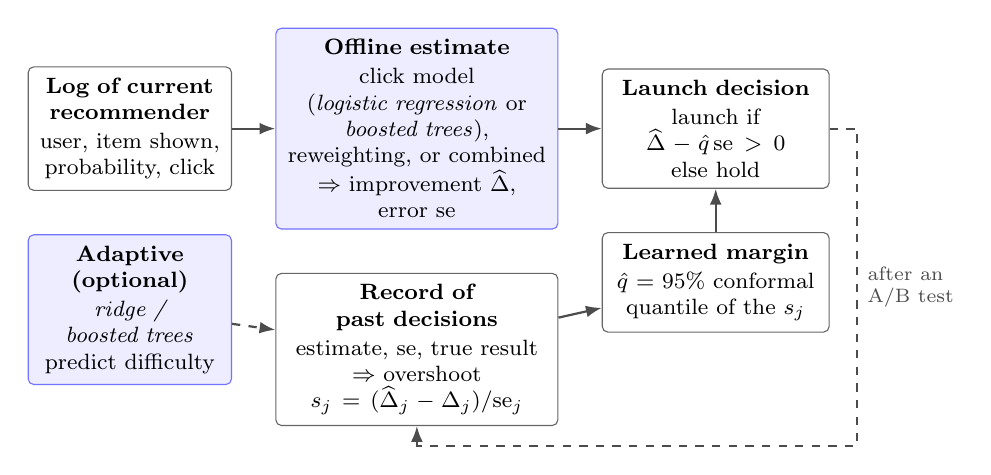
\begin{tikzpicture}[
  font=\footnotesize,
  box/.style={draw=black!60, rounded corners=2pt, align=center, inner sep=4pt, text width=#1},
  box/.default=2.6cm,
  ml/.style={box=#1, fill=blue!7, draw=blue!55},
  ml/.default=2.6cm,
  arr/.style={-{Latex[length=2mm]}, thick, black!70},
  node distance=0.45cm and 0.55cm]

\node[box=2.3cm] (log) {\textbf{Log of current\\recommender}\\[1pt]user, item shown,\\probability, click};
\node[ml=3.3cm, right=of log] (est) {\textbf{Offline estimate}\\[1pt]click model\\(\emph{logistic regression} or\\\emph{boosted trees}),\\reweighting, or combined\\[1pt]$\Rightarrow$ improvement $\widehat\Delta$,\\error $\mathrm{se}$};
\node[box=2.6cm, right=of est] (dec) {\textbf{Launch decision}\\[1pt]launch if\\$\widehat\Delta - \hat q\,\mathrm{se} > 0$\\else hold};

\node[box=3.3cm, below=0.55cm of est] (hist) {\textbf{Record of past decisions}\\[1pt]estimate, se, true result\\$\Rightarrow$ overshoot\\$s_j=(\widehat\Delta_j-\Delta_j)/\mathrm{se}_j$};
\node[box=2.6cm, below=0.55cm of dec] (q) {\textbf{Learned margin}\\[1pt]$\hat q$ = 95\% conformal\\quantile of the $s_j$};
\node[ml=2.3cm, below=0.55cm of log] (diff) {\textbf{Adaptive (optional)}\\[1pt]\emph{ridge / boosted trees}\\predict difficulty};

\draw[arr] (log) -- (est);
\draw[arr] (est) -- (dec);
\draw[arr] (hist) -- (q);
\draw[arr] (q) -- (dec);
\draw[arr, dashed] (diff) -- (hist);
\draw[arr, dashed] (dec.east) -- ++(0.35,0) |- node[pos=0.25, right, align=left, font=\scriptsize] {after an\\A/B test} ($(hist.south)+(0,-0.25)$) -- (hist.south);
\end{tikzpicture}

\caption{Overview. A classifier-based estimator turns the current recommender's log into an estimated improvement and its standard error. The record of past decisions gives the learned margin. Blue boxes contain the machine-learning models.}
\label{fig:pipeline}
\end{figure*}

\begin{table}[t]
\centering
\caption{Terms used in this paper}
\label{tab:terms}
\small
\begin{tabular}{p{0.3\columnwidth}p{0.6\columnwidth}}
\toprule
Term & Meaning \\
\midrule
Recommender & A model that chooses which items to show a user \\
Log & Records of what the current recommender showed and whether it was clicked \\
Offline estimate & Estimated click rate of a new recommender, computed from the current recommender's log \\
Improvement $\Delta$ & Click rate of new minus click rate of current recommender \\
Standard error (se) & The estimate's own report of how uncertain it is \\
Margin & Amount subtracted from the estimate before deciding; launch if estimate $-$ margin $>0$ \\
Coverage & How often the margin was large enough (estimate $-$ margin $\le$ true $\Delta$); target 95\% \\
Wrong launch & Launching a recommender that is not actually better \\
Power & How often a recommender that \emph{is} better gets launched \\
\bottomrule
\end{tabular}
\end{table}

\section{Related Work}
\textbf{Offline estimation for recommenders.} Estimating a new recommender's click rate from logs is studied as off-policy evaluation. Standard estimators reweight logged clicks~\cite{horvitz1952,swaminathan2015snips}, use a learned click model, or combine both~\cite{dudik2011dr,wang2017switch}. No single estimator is best everywhere, which has led to methods that \emph{choose} an estimator for each task~\cite{udagawa2023pasif,felicioni2024autoope}; we do not choose an estimator but make the decision reliable for whichever one is used. \textbf{Uncertainty for these estimates} is usually a normal-approximation or concentration bound~\cite{thomas2015hcope,maurer2009eb}, valid only when the estimator is unbiased; offline A/B testing~\cite{gilotte2018offlineab} and risk-aware selection~\cite{kiyohara2024sharpe} also rely on within-log variance. \textbf{Conformal prediction} gives distribution-free guarantees from a calibration set~\cite{vovk2005alrw,lei2018distfree} and extends to weighted and shifted settings~\cite{tibshirani2019covshift,barber2023beyond}. It has been used to give intervals for outcomes or values under a new recommender or policy from a single log~\cite{taufiq2022copp,zhang2023copp,foffano2023conformal}; we instead calibrate the \emph{launch decision} using a history of past decisions with known outcomes.

\section{Estimating a New Recommender Offline}
The current recommender $A$ produced a log of $n$ rows. In row $i$, a user with features $x_i$ was shown item $a_i$ with probability $p_i$, and a click $r_i\in\{0,1\}$ was recorded. The new recommender $B$ would show item $a$ with probability $\pi_B(a\mid x)$. We compare three ways to estimate $B$'s click rate; each gives one number $\phi_i$ per row, and the estimate is their average.

\textbf{Click model.} Train a classifier $\hat q(x,a)\approx P(\text{click}\mid x,a)$ on the log (logistic regression or gradient-boosted trees, with features for the user, item and position), then average its predictions over the items $B$ would show: $\phi_i = \sum_a \pi_B(a\mid x_i)\,\hat q(x_i,a)$. It is accurate only if the classifier is.

\textbf{Reweighting.} Count the logged clicks, but give more weight to items $B$ would show more often than $A$ did: $\phi_i = w_i r_i$ with $w_i = \pi_B(a_i\mid x_i)/p_i$. This is unbiased, because the reweighting exactly converts $A$'s choices into $B$'s on average, but it is noisy when weights are large.

\textbf{Combined.} Use the click model and reweight only its mistakes: $\phi_i = \sum_a \pi_B(a\mid x_i)\hat q(x_i,a) + w_i\big(r_i-\hat q(x_i,a_i)\big)$. This is unbiased when the probabilities $p_i$ are known, and less noisy than reweighting~\cite{dudik2011dr}.

Three common variants (self-normalised reweighting, self-normalised combined and a ``switch'' version that drops very large weights) gave the same conclusions; their results are in the code repository. The classifier is trained with 2-fold \emph{cross-fitting}, meaning it never predicts on rows it was trained on. All estimators were written from scratch and agree with the \texttt{obp} reference library~\cite{saito2021obd} to $10^{-9}$.

Since $A$'s own click rate is just the average logged click, the improvement estimate is $\Dhat = \frac1n\sum_i (\phi_i - r_i)$, with standard error $\se$ from the spread of $\phi_i - r_i$.

\section{The Learned Margin}
\textbf{Usual margin.} Launch if $\Dhat - z\,\se > 0$, with $z=1.645$ for 95\% safety. We also compare a conservative Bernstein bound~\cite{maurer2009eb} and, on real data, a standard error grouped (clustered) by hour~\cite{cameron2015cluster}.

\textbf{Learned margin.} Suppose we have $m$ past decisions with estimates $\Dhat_j$, standard errors $\se_j$ and true improvements $\Delta_j$ measured later. For each, record how many standard errors the estimate overshot the truth:
\begin{equation}
s_j = (\Dhat_j - \Delta_j)/\se_j .
\end{equation}
Sort the $s_j$ and take $\hat q$, the $\lceil (m+1)\cdot 0.95\rceil$-th smallest (or $+\infty$ if $m$ is too small). For a new decision, launch if
\begin{equation}
L = \Dhat - \hat q\,\se > 0 .
\end{equation}
If past estimates were honest, $\hat q\approx1.645$; on real data it was about 2.7. Fig.~\ref{fig:hist} shows why: on the real decisions, 19\% of estimates overshot the truth by more than 1.645 standard errors, almost four times the 5\% that the usual margin assumes.

\begin{figure}[t]
\centering
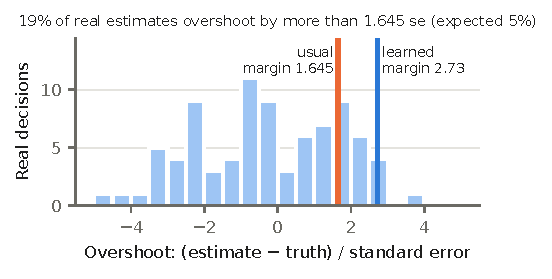
\includegraphics[width=\columnwidth]{../figures/error_histogram.pdf}
\caption{Overshoot scores $s_j$ of the 84 real decisions (combined estimator). The usual margin (orange) is passed far more often than 5\% of the time; the learned margin (blue) is set so that only 5\% lie beyond it.}
\label{fig:hist}
\end{figure}

\begin{proposition}
If the new decision is exchangeable with the past ones (it ``looks like'' them, with no systematic difference), then $\Pr(\Delta_{\mathrm{new}} \ge L) \ge 0.95$, whatever the estimator and even if it is biased.
\end{proposition}
\begin{proof}
$\Delta_{\mathrm{new}} \ge L$ exactly when $s_{\mathrm{new}} \le \hat q$. Under exchangeability every ranking of the $m+1$ scores is equally likely, so $s_{\mathrm{new}}$ lands above the chosen order statistic with probability at most 5\%~\cite{vovk2005alrw,lei2018distfree}.
\end{proof}
\noindent A wrong launch needs $L>0$ while $\Delta\le0$, so at most 5\% of decisions end in a wrong launch. The history grows with every A/B test (dashed arrow in Fig.~\ref{fig:pipeline}).

\textbf{Adaptive learned margin.} Some decisions are harder than others, for example when $B$ is very different from $A$ and the weights are large. The adaptive version trains a regression model (ridge regression or gradient-boosted trees) to predict how large $|s_j|$ will be from features known before the outcome: log size, the largest and average weight, the spread of the weights, the effective sample size and $\log\se$. Each score is divided by its predicted difficulty $\hat\sigma_j$ before taking the quantile, and the new margin becomes $\hat q\,\se\,\hat\sigma_{\text{new}}$, so easy decisions get a smaller margin. The model is trained with 5-fold cross-fitting so that no past decision's score trains the model that rescales it, in the spirit of CV+~\cite{barber2021jackknife}. A split version (fit on one third, calibrate on the rest) keeps the exact guarantee.

\section{Data and Experiments}
\textbf{Real data.} The Open Bandit Dataset~\cite{saito2021obd} contains about 26 million recommendations from a fashion e-commerce site over seven days in three campaigns (80, 34 and 46 items, three positions on the page). Two recommenders were run \emph{at the same time} on randomly split traffic: one shows items uniformly at random, the other adapts to recent clicks (Bernoulli Thompson sampling). Because they served the same population at the same time, each one's measured click rate is the true answer when estimating it from the other's log. We cut each campaign into fourteen 12-hour windows and make two decisions per window: estimating the adaptive recommender from the random one's log (the adaptive one is better in all but one window), and estimating the random recommender from the adaptive one's log (here the weights reach about 600). This gives 84 real decisions. The adaptive recommender's item probabilities are its observed item frequencies per hour and position. True improvements are about $\pm0.0015$ in click rate, with their own measurement error (about 0.0003) taken into account.

\textbf{Controlled experiments.} To test many decisions with exact truth, we turn six OpenML classification datasets (letter, pendigits, optdigits, satimage, mfeat-factors, segment) into recommendation problems~\cite{dudik2011dr}: classes are items, and a ``click'' happens with probability 0.9 for the correct class and 0.05 otherwise, so every recommender's true click rate can be computed exactly. The current recommender is a weak logistic-regression classifier. New recommenders are realistic small changes: retrained on new or larger data, more or less confident, more or less random exploration, or a different classifier (naive Bayes, $k$-nearest neighbours, random forest), plus two much stronger models. Of these, 27\% are not actually better. Half of the experiments add a population shift between the log and the deployment period, created along the first principal component (PCA). With two log sizes and four repeats this gives 448 experiments per dataset.

\textbf{How we test.} Each rule is judged on decisions it has not seen. Real data: each window uses only earlier windows as its history (and, separately, one campaign is tested using the other two). Controlled: $m\in\{20,50,100\}$ random experiments form the history and the rest are tested, over 100 random splits; we also use five datasets as the history and test on the sixth, and use a history without shift but test with shift.

\begin{table}[t]
\centering
\caption{How wrong the real estimates are compared with the error they report (84 real decisions; bias and RMSE in units of $10^{-4}$ click rate). Inflation $=$ actual spread of errors / reported standard error, using the usual, page-grouped or hour-grouped standard error. 1.0 means the reported error is honest.}
\label{tab:inflation}
\small
\setlength{\tabcolsep}{4pt}
\begin{tabular}{lrrrrrr}
\toprule
& & & & \multicolumn{3}{c}{Inflation}\\
\cmidrule(lr){5-7}
Estimator & Bias & RMSE & se & Usual & Page & Hour\\
\midrule
Click model (LR) & -0.2 & 10.7 & 2.5 & 2.57 & 2.38 & 1.96\\
Click model (GBT) & +0.0 & 10.9 & 2.5 & 2.62 & 2.41 & 1.99\\
Reweighting & +1.5 & 13.6 & 6.9 & 1.67 & 1.62 & 1.22\\
Combined (GBT) & -0.7 & 16.1 & 7.4 & 1.80 & 1.76 & 1.13\\
\bottomrule
\end{tabular}
\end{table}


\begin{figure}[t]
\centering
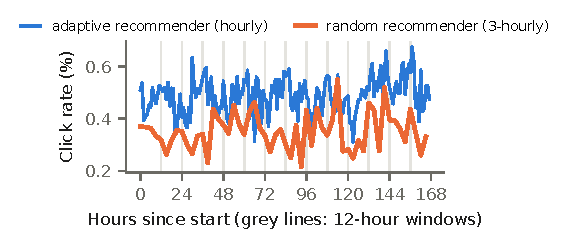
\includegraphics[width=\columnwidth]{../figures/hourly_drift.pdf}
\caption{Click rate of the two recommenders by hour (``all items'' campaign). Behaviour changes within each 12-hour window, which a standard error that treats every row as independent does not capture.}
\label{fig:drift}
\end{figure}

\begin{figure*}[t]
\centering
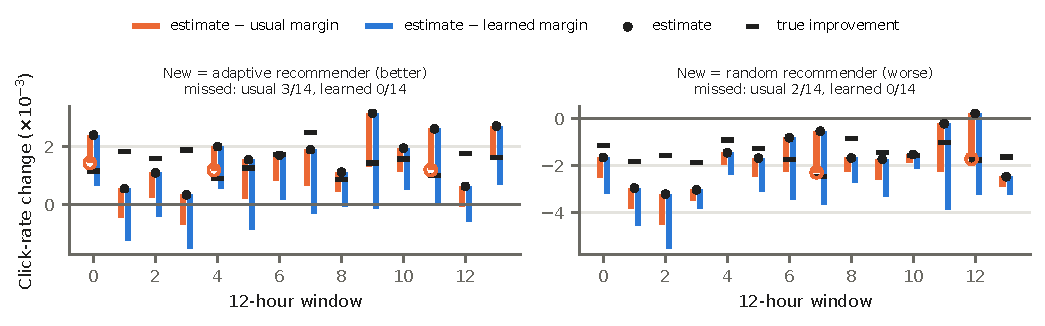
\includegraphics[width=\textwidth]{../figures/decision_chart.pdf}
\caption{Every real decision in the main (``all items'') campaign. Bars run from the estimate down to estimate $-$ margin; launch if the bottom of the bar is above zero. A circle marks a miss: the true improvement lies below the bar. The learned margin here is computed from the other two campaigns. Across all three campaigns the usual margin misses 16 of 84 decisions and the learned margin 4 of 84.}
\label{fig:decisions}
\end{figure*}

\begin{table*}[t]
\centering
\caption{Main results. Coverage: how often estimate $-$ margin was below the true improvement (target 0.95; values at or above it in bold). Power: how often a better recommender was launched. Usual: 1.645 standard errors; Hour: usual margin with hour-grouped standard errors (real data only); Bern.: Bernstein bound; Ours: learned margin.}
\label{tab:results}
\small
\begin{tabular}{lrrrrrrrr}
\toprule
& \multicolumn{4}{c}{Coverage} & \multicolumn{4}{c}{Power} \\
\cmidrule(lr){2-5}\cmidrule(lr){6-9}
Estimator & Usual & Hour & Bern. & Ours & Usual & Hour & Bern. & Ours \\
\midrule
\multicolumn{9}{l}{\emph{Real data (60 decisions, history = earlier windows)}} \\
Click model (LR) & .617 & .717 & .833 & \textbf{.967} & .833 & .800 & .667 & .467 \\
Click model (GBT) & .600 & .650 & .767 & \textbf{.967} & .800 & .667 & .667 & .133 \\
Reweighting & .767 & .900 & \textbf{1.00} & \textbf{.983} & .700 & .567 & .033 & .300 \\
Combined (GBT) & .800 & .900 & \textbf{1.00} & \textbf{.983} & .667 & .567 & .033 & .267 \\
\midrule
\multicolumn{9}{l}{\emph{Controlled experiments (exact truth, $m=50$ past decisions)}} \\
Click model (LR) & .748 & -- & .810 & \textbf{.962} & .111 & -- & .024 & .001 \\
Click model (GBT) & .675 & -- & .790 & \textbf{.961} & .742 & -- & .650 & .293 \\
Reweighting & .870 & -- & \textbf{.968} & \textbf{.961} & .941 & -- & .745 & .807 \\
Combined (GBT) & .913 & -- & \textbf{.988} & \textbf{.960} & .885 & -- & .616 & .808 \\
\bottomrule
\end{tabular}
\end{table*}


\begin{figure}[t]
\centering
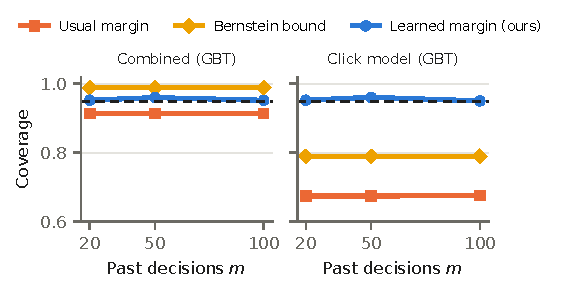
\includegraphics[width=\columnwidth]{../figures/coverage_vs_history.pdf}
\caption{Controlled experiments: coverage against the number of past decisions. The learned margin meets the 0.95 target from $m=20$; the usual margin stays below it for both estimators.}
\label{fig:history}
\end{figure}

\begin{figure}[t]
\centering
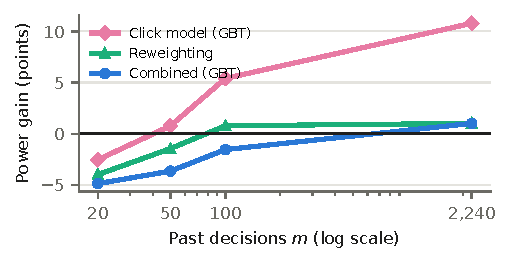
\includegraphics[width=\columnwidth]{../figures/adaptive_gain.pdf}
\caption{Adaptive learned margin (boosted-tree difficulty model): power gained over the plain learned margin. Below 0 it hurts, above 0 it helps; it pays off only with a large history ($m{=}2{,}240$ uses five other datasets). A ridge difficulty model behaves similarly. Coverage stays within 0.91--1.00.}
\label{fig:adaptive}
\end{figure}

\section{Results}
\textbf{Real estimates are about twice as wrong as they claim.} Table~\ref{tab:inflation} compares the actual spread of errors with the reported standard error. Average bias is small, but errors are 1.7--1.8$\times$ larger than reported for reweighting and combined estimators and 2.6$\times$ for click models. To find out why, we recomputed standard errors in groups. Grouping the three items shown together on one page changes almost nothing, so that is not the cause. Grouping by hour explains most of the gap for reweighting and combined estimators (1.1--1.3$\times$): user behaviour drifts from hour to hour within a window, which Fig.~\ref{fig:drift} shows directly. Click models stay near 2$\times$ because their error is \emph{bias} from an imperfect classifier, which no standard-error formula can see.

\textbf{The learned margin is safe on real data.} Fig.~\ref{fig:decisions} shows every decision in the main campaign and Table~\ref{tab:results} summarises all of them: the usual margin is large enough only 60--80\% of the time, and even the hour-grouped version only 65--90\%. The Bernstein bound is safe for reweighting and combined estimators but so cautious that it launches the better recommender in at most 3\% of cases. The learned margin is safe 95--98\% of the time for every estimator, both when using earlier windows and when using other campaigns as history. It launches better recommenders less often than the usual margin (13--47\% versus 63--83\%); this is the cost of being honest about real uncertainty.

\textbf{Controlled experiments.} Table~\ref{tab:results} and Fig.~\ref{fig:history}: the usual margin's coverage ranges from 0.675 to 0.913, and with the boosted-tree click model it launches 27.7\% of recommenders that are not better. The learned margin reaches 0.950--0.962 for all ten estimator variants and all history sizes, and that click model's wrong launches drop to 0\%. For the combined estimator, power falls from 0.885 to 0.808, much less than the Bernstein bound's drop to 0.616. Using five other datasets as the history still gives 0.93--0.95 coverage, and the learned margin is already valid with 20 past decisions.

\textbf{Adaptive margin.} Fig.~\ref{fig:adaptive}: the learned difficulty model needs data. With 20 past decisions it costs 2.5--7 points of power; at 50 the two versions are close; at 100 it helps the boosted-tree click model (up to $+5.4$); and with a large history ($\approx2{,}240$ decisions) it gains 1 point for the reweighting and combined estimators and 9--11 points for that click model, whose difficulty varies the most; on the small real history it mostly loses power.

\textbf{When it breaks.} If the history has no population shift but the new decisions do, coverage falls to 0.78--0.88 for unbiased estimators: the past no longer describes the present, which violates the assumption of the guarantee.

\section{Discussion and Limitations}
The learned margin changes the question from ``is my estimator unbiased?'' to ``how wrong has my process been on decisions like this?''. It needs only a stored record of offline estimates and later real results, works with any estimator, and needs no explanation of why errors are large. Our real ground truth comes from only two recommenders, so the real decisions share structure and the ``not better'' cases are clear-cut. The click probabilities in the controlled experiments are deliberately simple. Honest margins also mean fewer launches, and the adaptive version only pays off with a large history.

\section{Conclusion}
Offline launch decisions are only as safe as their margin. On real logs the usual margin was too small by a factor of about two, partly because of hourly drift and partly because of click-model bias. Setting the margin from a record of past decisions restored the promised safety level on real and controlled data, using only classical models. Future work includes weighting past decisions by similarity and combining the learned margin with hour-grouped standard errors.

\bibliographystyle{IEEEtran}
\bibliography{references}
\end{document}
